%--------------------------------------------------------------------------------------------------
% elasticity.tex
%
% This document define the frontespiece of the presentation
%
% author: Andrea Meneghinello
% version: 0.1
%--------------------------------------------------------------------------------------------------
\section{Elasticity}
\begin{frame}{Elasticity}
	\begin{columns}
		\begin{column}{0.5\textwidth}
			\textbf{elasticity} obtained by
			\begin{itemize}
				\item{\footnotesize{how PaaS exploits IaaS assets}}
				\begin{itemize}
					\item{\scriptsize{computing}}
					\item{\scriptsize{storage}}
					\item{\scriptsize{networking}}
				\end{itemize}
				\item{\footnotesize{how we build our services}}
				\begin{itemize}
					\item{\scriptsize{software architectures}}
					\item{\scriptsize{Software Engineering principles}}
				\end{itemize}
			\end{itemize}
		\end{column}
		\begin{column}{0.5\textwidth}
			\begin{figure}
				\centering{}
				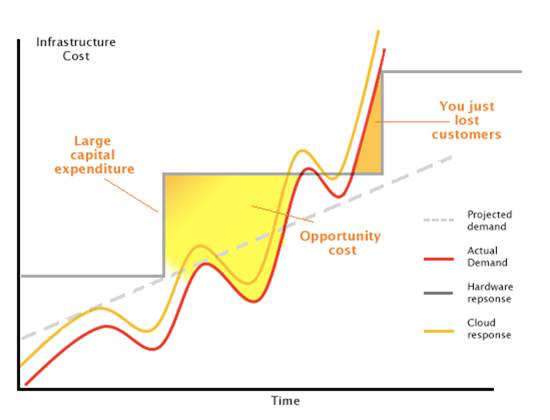
\includegraphics[scale=0.35]{images/elasticity.png}
			\end{figure}
			\begin{flushright}
				\tiny{source: \url{https://goo.gl/EzhyD5}}
			\end{flushright}
		\end{column}
	\end{columns}
\end{frame}

\subsection{Requirements}
\begin{frame}{Requirements}
	\only<1>
	{
		\begin{columns}
			\begin{column}{0.6\textwidth}
				elasticity major requirements
				\begin{itemize}
					\item{\footnotesize{from definition of elasticity}}
					\begin{itemize}
						\item{\scriptsize{autonomy}}
						\item{\scriptsize{scalability $\rightarrow{}$ \textbf{focus on horizontal}}}
						\item{\scriptsize{adaptability}}
					\end{itemize}
					\item{\footnotesize{specific for PaaS layer}}
					\begin{itemize}
						\item{\scriptsize{SLA-awareness}}
						\item{\scriptsize{composability}}
						\item{\scriptsize{service continuity in SW upgrades}}
					\end{itemize}
				\end{itemize}
			\end{column}
			\begin{column}{0.4\textwidth}
				\begin{figure}
					\centering{}
					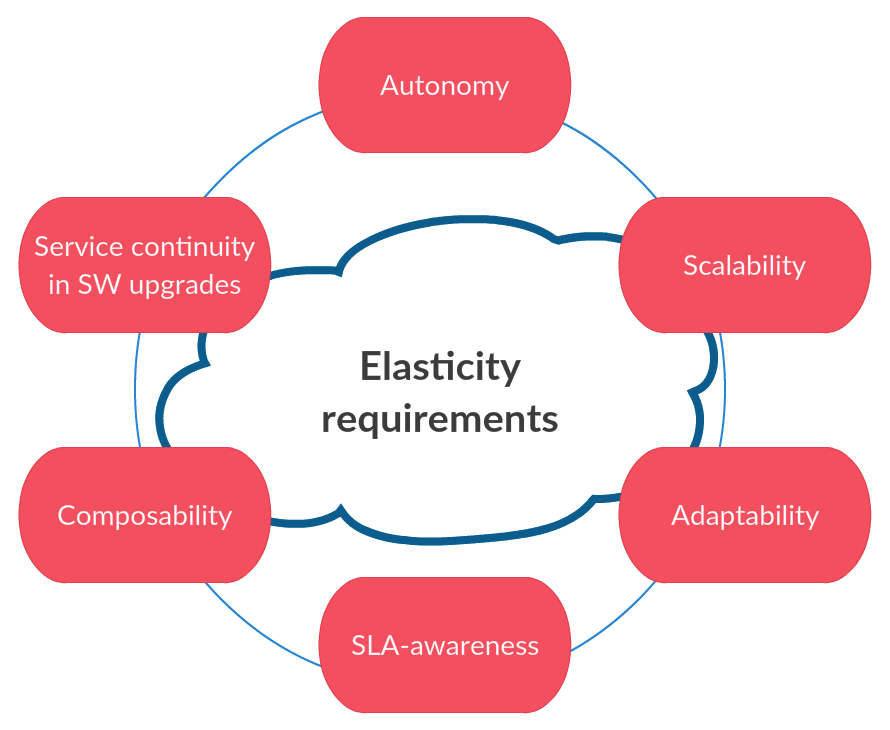
\includegraphics[scale=0.14]{images/elasticity-requirements.png}
				\end{figure}
			\end{column}
		\end{columns}
	}
	\only<2>
	{
		\begin{columns}
			\begin{column}{0.65\textwidth}
				scalability
				\begin{itemize}
					\item{\footnotesize{\textbf{replication (horizontal)}}}
					\begin{itemize}
						\item{\scriptsize{the only possible solution in PaaS}}
						\item{\scriptsize{PaaS manages units of deployments}}
					\end{itemize}
					\item{\footnotesize{some components are replicated when necessary}}
					\begin{itemize}
						\item{\scriptsize{the process must be transparent}}
						\item{\scriptsize{services must be well-designed}}
						\item{\scriptsize{classic architectures does not help}}
					\end{itemize}
					\item{\footnotesize{other}}
					\begin{itemize}
						\item{\scriptsize{redimension (vertical)}}
						\item{\scriptsize{migration}}
					\end{itemize}
				\end{itemize}
			\end{column}
			\begin{column}{0.35\textwidth}
				\begin{figure}
					\centering{}
					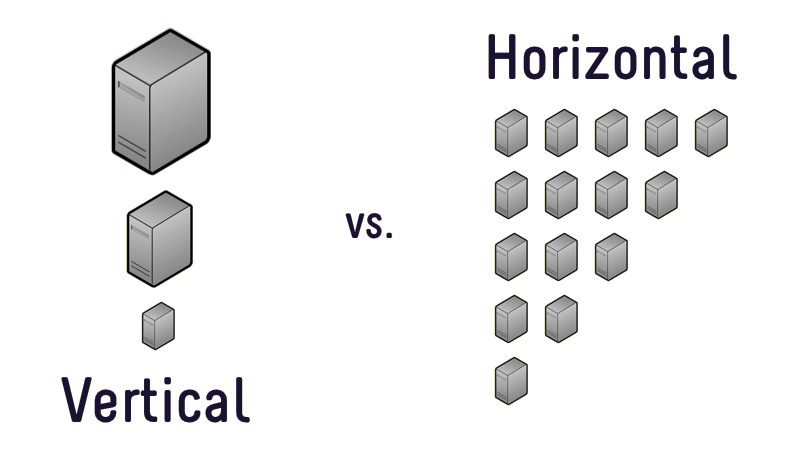
\includegraphics[scale=0.15]{images/scalability.png}
				\end{figure}
				\begin{flushright}
					\tiny{source: \url{https://goo.gl/orFWSi}}
				\end{flushright}
			\end{column}
		\end{columns}
	}
\end{frame}

\subsection{Multi-tenancy}
\begin{frame}{Multi-tenancy}
	\only<1>
	{
		\begin{columns}
			\begin{column}{0.57\textwidth}
				requirements
				\begin{itemize}
					\item{\footnotesize{availability $\rightarrow{}$ redundant services}}
					\item{\footnotesize{secure tenants isolation}}
					\item{\footnotesize{guarantee of service $\rightarrow$ performance}}
					\item{\footnotesize{management of underlying resources}}
				\end{itemize}
				\begin{center}
					providers have to plan SLA with a rich set of \textbf{objectives}
				\end{center}
			\end{column}
			\begin{column}{0.43\textwidth}
				\begin{figure}
					\centering{}
					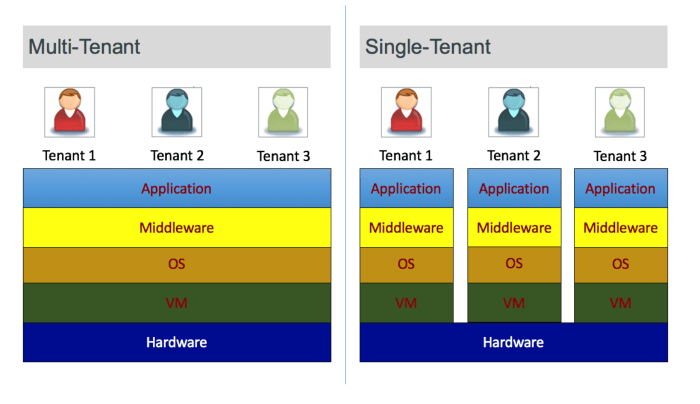
\includegraphics[scale=0.21]{images/multi-tenancy.png}
				\end{figure}
				\begin{flushright}
					\tiny{source: \url{http://goo.gl/MlsmWj}}
				\end{flushright}
			\end{column}
		\end{columns}
	}
	\only<2>
	{
		\begin{columns}
			\begin{column}{0.57\textwidth}
				naive architectures lead to
				\begin{itemize}
					\item{\footnotesize{inflexibility toward different needs}}
					\item{\footnotesize{security lacks}}
					\item{\footnotesize{inadequate usability}}
					\begin{itemize}
						\item{\scriptsize{sustain high workload $\rightarrow{}$ elasticity}}
					\end{itemize}
				\end{itemize}
			\end{column}
			\begin{column}{0.43\textwidth}
				\begin{figure}
					\centering{}
					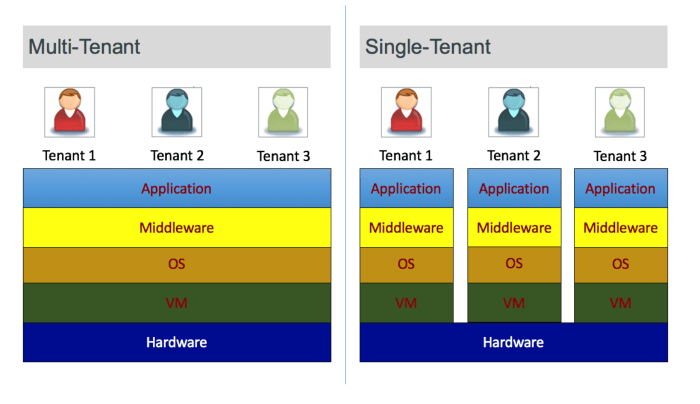
\includegraphics[scale=0.21]{images/multi-tenancy.png}
				\end{figure}
				\begin{flushright}
					\tiny{source: \url{http://goo.gl/MlsmWj}}
				\end{flushright}
			\end{column}
		\end{columns}
	}
\end{frame}